% Primera entrega — propuesta. Compila: pdflatex slides_primera_entrega.tex (2 veces)
\documentclass[aspectratio=169,10pt]{beamer}
\usepackage[spanish]{babel}
\usepackage{booktabs}
\usepackage{graphicx}
\usepackage{hyperref}
\usetheme{default}
\usecolortheme{seahorse}
\title{Triage de alertas SOC sobre 2M de eventos con modelos tabulares, de texto y de grafo}
\subtitle{Propuesta de proyecto — Aprendizaje Automático (Primera entrega)}
\author{Author Name}
\date{8va sesión · 15 min + 5 min preguntas}

\begin{document}
\frame{\titlepage}

\begin{frame}{Índice}
\tableofcontents
\end{frame}

\section{Introducción}
\begin{frame}{1. Contexto}
\begin{itemize}
\item Un SOC vigila con decenas de productos: firewalls, EDR, identidad, nube, hipervisores, DNS.
\item WitFoo Precinct normaliza y correlaciona con \textbf{261 reglas de detección}; agrupa se\~nales en \textbf{incidentes} (se\~nales + subgrafo de proveniencia + reporte).
\item Dataset: \texttt{precinct6-cybersecurity} v2.1.0 — \textbf{2,011,674 eventos} en 6 días (26 jul--01 ago 2024), 4 organizaciones, 19 productos, 12 fabricantes.
\end{itemize}
\end{frame}

\begin{frame}{1. Motivación}
\begin{itemize}
\item \textbf{Volumen}: 2M de eventos en 6 días, imposible a mano.
\item \textbf{Desbalance extremo}: 0.38\% malicioso (IR 245:1) $\to$ accuracy miente (94.31\% con siempre-benigno).
\item \textbf{Asimetría de costos}: FN (brecha) $>>$ FP $\to$ optimizar recall minoritario, no exactitud.
\item \textbf{Contexto del analista}: decidir exige mensaje + MITRE + cadena, no un n\'umero.
\end{itemize}
\end{frame}

\begin{frame}{1. Pregunta de investigación}
\textbf{Objetivo}: estimar el nivel de riesgo de un evento con probabilidades calibradas y recomendación operativa.

\begin{quote}
¿Es posible recuperar eventos maliciosos con desbalance 245:1 y deriva temporal combinando representaciones tabulares, textuales y estructurales, y qué compromiso existe con el nivel intermedio?
\end{quote}

Específicos: (i) caracterizar datos y leakage; (ii) $\ge$5 preprocesos; (iii) 3 modelos con complejidad; (iv) desplegar servicio + consola.
\end{frame}

\section{Trabajo previo}
\begin{frame}{2. Marco de referencia}
Tres familias:
\begin{itemize}
\item \textbf{Grafos de proveniencia}: NODLINK (APT online), KnowHow (CTI interpretable), FLASH (GNN temporal), threaTrace/GraphSAGE (nivel de nodo).
\item \textbf{Mapeo a ATT\&CK desde texto}: TRAM (MITRE, + notebooks SciBERT), comparativas TF-IDF vs transformers.
\item \textbf{Desbalance}: Focal Loss; formulaciones sensibles al costo (FN $>>$ FP).
\end{itemize}
Dos casos se analizan en detalle, uno por estructura y otro por texto.
\end{frame}

\begin{frame}{2. Caso 1: Devign (NeurIPS 2019)}
\textbf{Enfoque}: GNN (GGNN + módulo Conv) sobre representación compuesta del código (AST + dependencias de control/datos). Tarea: \textbf{binaria a nivel función} (¿vulnerable?).
\begin{itemize}
\item \textbf{Datos}: etiquetados manualmente, $\sim$600 h-persona, 4 librerías C (Linux, QEMU, Wireshark, FFmpeg); código real complejo.
\item \textbf{Resultado}: \textbf{+10.51\% accuracy / +8.68\% F1} vs baselines; +27.99\% F1 vs analizadores estáticos; 74.11\% en 40 CVEs nuevos.
\end{itemize}
Lección: precedente del componente de grafo. Contraste: etiquetas caras/limpias vs nuestras automáticas/ruidosas.
\end{frame}

\begin{frame}{2. Caso 2: CVSS-BERT (IEEE ICMLA 2021)}
\textbf{Enfoque}: trabaja con \textbf{texto, no código}. \textbf{8 clasificadores BERT}, uno por métrica del vector CVSS, desde la descripción del CVE (45,926 CVEs 2018--2020).
\begin{itemize}
\item \textbf{Motivación}: al publicarse una vuln solo hay descripción; el análisis experto tarda días.
\item \textbf{Resultado}: accuracy 83.79--96.07\% por métrica; severidad MAE 0.73, 55.3\% match exacto $\to$ muy cerca del experto. Incluye saliency explicable.
\item \textbf{Limitación}: los puntajes CVSS \textbf{varían según quién asigna} (hasta 0.8 pts NVD vs otros; 1.3 por versión; degradación aguas abajo hasta 77\%) $\to$ etiquetas dependen del contexto.
\end{itemize}
Lección: precedente del componente de texto; su límite fundamenta nuestras limitaciones.
\end{frame}

\begin{frame}{2. Síntesis y brecha}
\begin{table}\small
\begin{tabular}{@{}llll@{}}
\toprule
 & Devign & CVSS-BERT & Propuesto \\
\midrule
Entrada & grafo código & texto CVE & tabular + texto + subgrafo \\
Tarea & binaria & 8 métricas $\to$ puntaje & 3 niveles + ATT\&CK \\
Etiquetas & manuales 600\,h & NVD experto & Precinct automático \\
Se\~nal & +10.51\% acc & MAE 0.73 & cascada + compromiso \\
\bottomrule
\end{tabular}
\end{table}
\textbf{Brecha}: la literatura opera sobre código o descripciones de vulnerabilidades, no sobre telemetría de operación en tiempo real con desbalance extremo, deriva temporal y humano en el bucle.
\end{frame}

\section{Metodología}
\begin{frame}{3. Definición del problema}
\textbf{Clasificación supervisada multiclase}: $f: x \mapsto (y, p)$ con $y \in \{$benign, suspicious, malicious$\}$.

Representación $x$ en tres niveles:
\begin{itemize}
\item campos tabulares del evento;
\item mensaje crudo saneado;
\item subgrafo de vecindario temporal ($\pm$5 min).
\end{itemize}
Condicionantes: desbalance 245:1, distribución no estacionaria, humano en el bucle.
\end{frame}

\begin{frame}{3. Dataset y exploración}
\begin{table}\small
\begin{tabular}{@{}lrr@{}}
\toprule
Nivel & Eventos & \% \\
\midrule
benign & 1,897,153 & 94.31 \\
suspicious & 106,793 & 5.31 \\
malicious & 7,728 & 0.38 \\
\bottomrule
\end{tabular}
\end{table}
Además: 238,511 se\~nales históricas, 47,585 nodos / 1,740,438 aristas, 51,371 incidentes con reporte.
\begin{center}
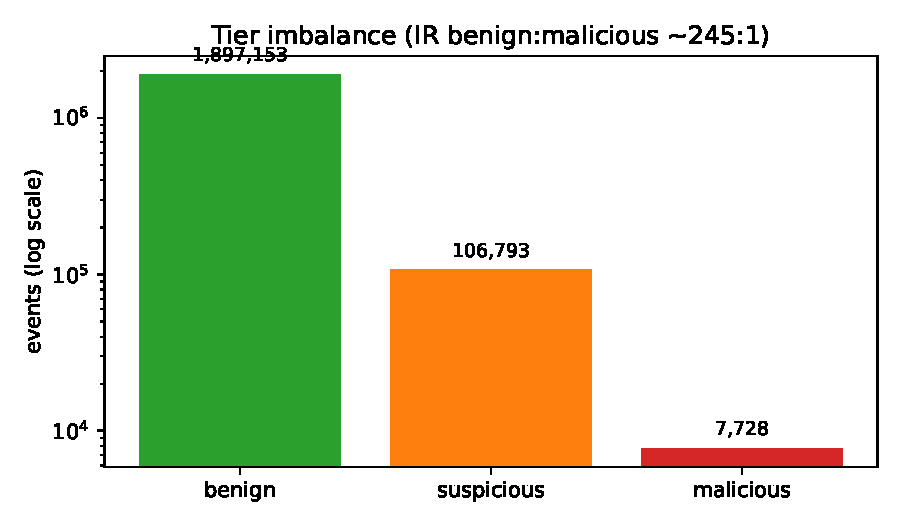
\includegraphics[width=0.38\linewidth]{figures/label_distribution.pdf}
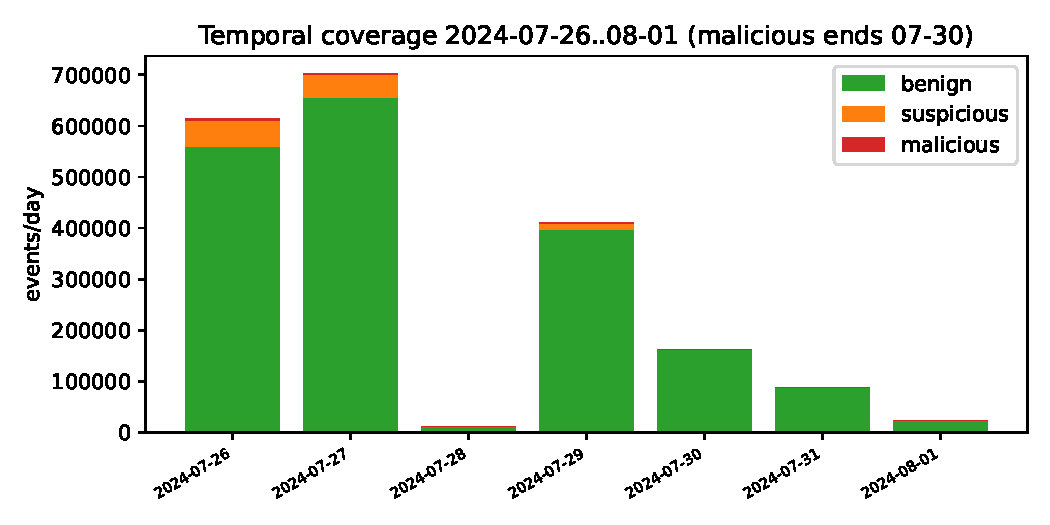
\includegraphics[width=0.38\linewidth]{figures/temporal_volume.pdf}
\end{center}
\end{frame}

\begin{frame}{3. Preprocesamiento (P1--P5)}
\begin{itemize}
\item \textbf{P1} Codificación categórica consciente del saneamiento (ausentes = nivel propio, no mediana).
\item \textbf{P2} Características temporales + partición temporal anti-leakage.
\item \textbf{P3} Desbalance: muestreo estratificado + ponderación de clases (sin SMOTE sobre codificadas).
\item \textbf{P4} Vectorización del texto del registro (TF-IDF 5k).
\item \textbf{P5} Subgrafo de vecindario $\pm$5 min por host/credencial.
\end{itemize}
Cumple el requisito de al menos tres metodologías.
\end{frame}

\begin{frame}{3. Modelos y complejidad}
\begin{itemize}
\item \textbf{M1 tabular} (gradient boosting, ponderado): fit crece con árboles$\times$filas$\times$características; inferencia = recorrido raíz-hoja.
\item \textbf{M2 texto}: concatena vectorización del mensaje + tabular; costo extra lineal en longitud del mensaje.
\item \textbf{M3 grafo}: agrega vecindario en ventana y alimenta clasificador; costo por evento según tama\~no del vecindario.
\end{itemize}
\textbf{Cascada de servicio}: M1 ordena la cola $\to$ M2 confirma con evidencia textual $\to$ M3 confirma con evidencia estructural.
\end{frame}

\begin{frame}{3. Diagrama del proceso}
\begin{center}
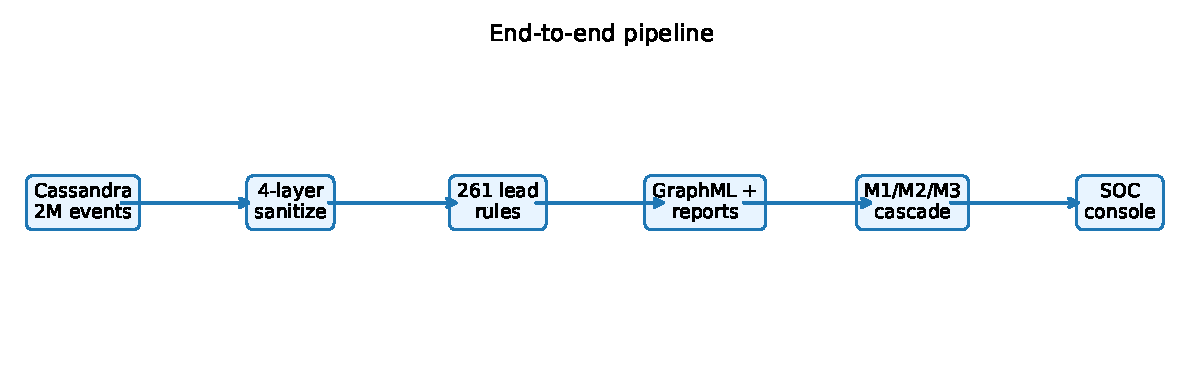
\includegraphics[width=0.9\linewidth]{figures/architecture.pdf}
\end{center}
Desde la captura y saneamiento, pasando por las 261 reglas y el preprocesamiento, hasta la cascada de modelos y la consola del analista.
\end{frame}

\begin{frame}{3. Protocolo de evaluación}
\begin{itemize}
\item \textbf{Partición temporal}: entrenar con el pasado, evaluar con el futuro (corte = cuantil 80 de la marca de tiempo).
\item \textbf{Métricas}: F1-macro y \'area bajo precisi\'on-recuerdo por clase; recall malicioso a FPR fijo.
\item La exactitud se reporta solo para mostrar que no es informativa bajo IR 245:1.
\item Se documentarán semillas e infraestructura para permitir replicación.
\end{itemize}
\end{frame}

\section{Experimentos}
\begin{frame}{4. Experimentos planeados}
\begin{itemize}
\item \textbf{E1 (base tabular)}: M1 sobre campos. Hipótesis: recupera benign/suspicious, colapsa en malicious $\to$ l\'inea base honesta.
\item \textbf{E2 (texto)}: M2 + mensaje. Hip\'otesis: eleva sustancialmente el recall malicioso (vocabulario de explotaci\'on).
\item \textbf{E3 (estructura)}: M3 + vecindario. Hip\'otesis: iguala E2 por mecanismo distinto y refleja movimiento lateral.
\end{itemize}
\textbf{Ablaciones}: (i) codificaci\'on del texto (frecuencias vs contextual); (ii) radio de la ventana temporal.
\end{frame}

\begin{frame}{4. Análisis previsto y despliegue}
\begin{itemize}
\item Matriz de confusi\'on normalizada por fila: hacia qu\'e clase se desplaza el error minoritario.
\item Explicitar el \textbf{compromiso}: recuperar la clase minoritaria vs preservar el nivel intermedio.
\item \textbf{Despliegue}: servicio FastAPI en :8000 (\texttt{/score}, \texttt{/queue}, \texttt{/incident}) + consola React en el mismo origen (Docker multi-stage), con bit\'acora de feedback para re-entrenar.
\end{itemize}
\end{frame}

\section{Conclusión}
\begin{frame}{5. Limitaciones y trabajo futuro}
\textbf{Limitaciones previstas}
\begin{itemize}
\item Etiquetas de correlación automática, no de analista (oráculo imperfecto; mayoría sin procesar).
\item Distribución desigual por tiempo y organización $\to$ generalización restringida.
\item Análogo a CVSS: la etiqueta \textbf{depende del asignador} y su contexto.
\end{itemize}
\textbf{Trabajo futuro}
\begin{itemize}
\item Predicción multi-etiqueta de técnicas ATT\&CK.
\item Codificadores contextuales entrenables sobre los reportes de incidente.
\end{itemize}
\end{frame}

\begin{frame}{Referencias}
\tiny
Devign (NeurIPS 2019, arXiv:1909.03496) · CVSS-BERT (ICMLA 2021, arXiv:2111.08510) ·
Schwab \& Gwerder (Berna, 2020) · LADC 2024 (doi 10.1145/3697090.3697109) ·
arXiv:2112.10356 · NODLINK (2311.02331) · KnowHow (2509.05698) · FLASH (S\&P 2024) ·
threaTrace (2111.04333) · GraphSAGE (1706.02216) · TRAM (MITRE CTID) ·
TF-IDF vs transformers (2407.06753) · Focal Loss (1708.02002) ·
Cost-sensitive IDS (0807.2043) · ATT\&CK \url{https://attack.mitre.org/} ·
Dataset \url{https://huggingface.co/datasets/witfoo/precinct6-cybersecurity}
\end{frame}

\end{document}
